\chapter{Conceitos Básicos}
Este capítulo tem como objetivo apresentar alguns conceitos utilizados como base para a realização do presente trabalho. Algumas tecnologias serão expostas para facilitar o entendimento dos próximos capítulos. Também é discutido onde foi feito a utilização destas ferramentas e teorias no decorrer do trabalho, bem como as dificuldades encontradas.
% *************
% Métodos Ágeis
% *************
\section{Métodos Ágeis de Desenvolvimento de Software}

% *****
% Agile
% *****
\subsection{Agile}
\textit{Agile} (desenvolvimento ágil de software ou métodos ágeis) é um termo que se refere a abordagem de desenvolvimento de software em que requisitos e soluções evoluem através de um esforço colaborativo de times auto-geridos e multi-funcionais, de sues clientes e usuários finais. O conceito prega planejamentos adaptativos, desenvolvimento iterativo com melhorias contínuas e encoraja a rápida e flexível resposta a mudanças. O conceito é frequentemente posto em prática com o uso de frameworks de desenvolvimento, como \textit{Scrum} e \textit{Kanban}. O termo foi popularizado através do manifesto ágil de desenvolvimento de software \todo{citar agile-manifest}, que tem como valores:

\begin{itemize}
    \item Indivíduos e iterações mais que processos e ferramentas
    \item Software funcional mais que documentação abrangente
    \item Colaboração do cliente mais que negociação de contratos
    \item Responder a mudanças mais que seguir um plano
\end{itemize}

% *****
% Scrum
% *****
\subsection{Scrum}
\begin{figure}[h]
    \centering
    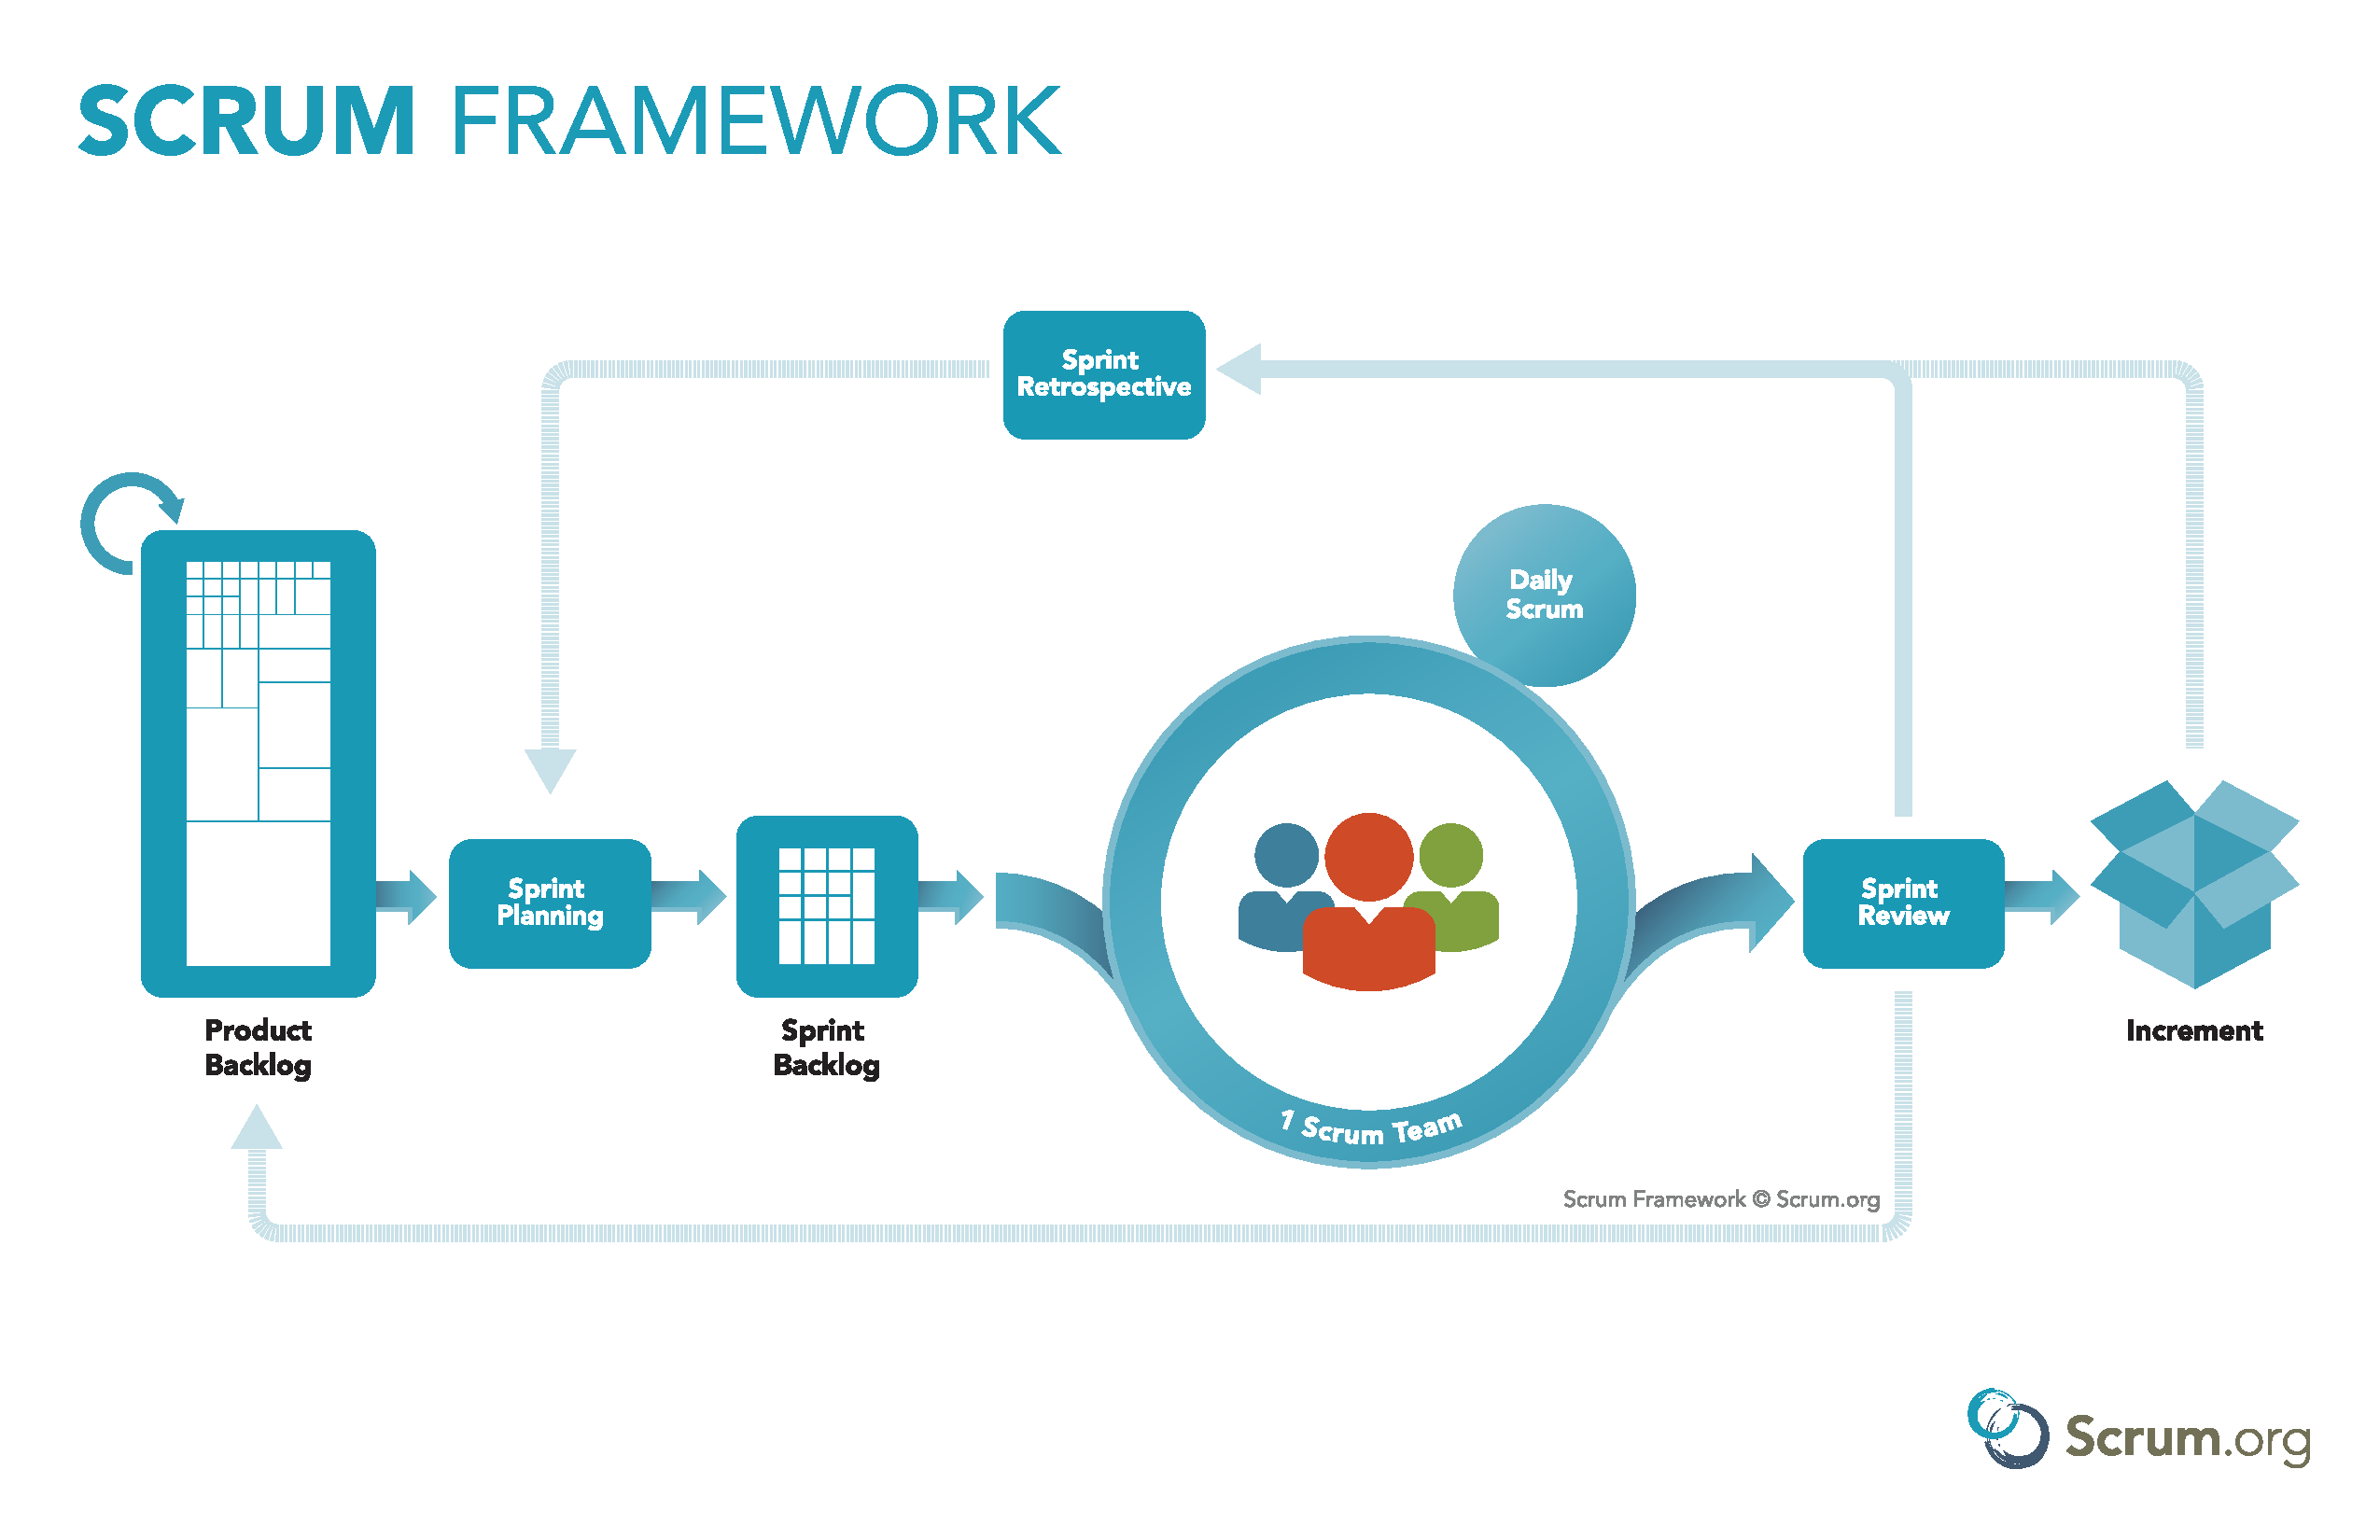
\includegraphics[width=\textwidth]{pfc/figuras/scrum.pdf}
    \caption{Estrutura do Scrum}
    \label{fig:scrum}
\end{figure}

\textit{Scrum} (Figura \ref{fig:scrum}) \todo{citar scrum-guide} é um framework com o propósito de abordar problemas adaptativos complexos. Ele não é um processo, técnica ou método definitivo, mas sim uma estrutura para empregar vários processos e técnicas. O framework fundamenta-se nos conceitos de transparência, inspeção e adaptação e tem como valores: compromisso, coragem, foco, abertura e respeito.

O \textit{Scrum} consiste em times com atribuições associadas, eventos e artefatos. Estes elementos são elencados a seguir:
\begin{itemize}
    \item Atribuições nos times:
    \begin{itemize}
        \item \textit{Product Owner}: responsável por maximizar o valor do produto resultante do trabalho do time de desenvolvimento. É uma única pessoal responsável por gerenciar o backlog do produto (\textit{Product Backlog}).
        \item \textit{Development Team}: é o time de desenvolvimento. Estes devem ter seus respectivos trabalhos auto-geridos de tal forma a aumentar a eficiência e eficacia do projeto.
        \item \textit{Scrum Master}: responsável por promover e dar apoio as regras do \textit{Scrum} dentro do time. Esta pessoa deve ajudar os demais a compreender a teoria por trás do framework, práticas, regras e valores.
    \end{itemize}
    \item Eventos:
    \begin{itemize}
        \item \textit{Sprint}: é o evento central do \textit{Scrum}, consistindo de uma janela limitada de tempo com duração de um mês ou menos. Durante este período temporal, a equipe deve concluir um versão incremental do produto a ser entregue. As durações das \textit{sprints} devem ser consistentes ao longo do projeto, com uma \textit{sprint} iniciando-se imediatamente ao término da anterior.
        \item \textit{Sprint Planning}: o trabalho a ser realizado durante a \textit{sprint} é planejado durante a sessão de \textit{sprint planning} através do trabalho colaborativo de todos os membros do time. A duração deste evento deve ser limitado proporcionalmente ao tamanho da janela de tempo da \textit{sprint}, sendo $8h$ o limite para uma sprint de um mês
        \item \textit{Daily Scrum}: é um evento diário executado pelo time de desenvolvimento, limitado a quinze minutos. Ocorre todos os dias no mesmo horário com o objetivo de inspecionar o trabalho executado no dia anterior e anteceder discussões sobre o trabalho futuro.
        \item \textit{Sprint Review}: evento que ocorre ao final da \textit{sprint} com o intuito de avaliar o progresso do time em relação ao incremento do produto. Durante a sessão, limita a $4h$ para uma \textit{sprint} de um mês, o time e \textit{stakeholders} discutem o que foi feito e proveem feedback.
        \item \textit{Sprint Retrospective}: evento que ocorre após a \textit{sprint review} e antecede a \textit{sprint planning}, limitado a $3h$ para uma \textit{sprint} de um mês. Durante o evento, o time tem a oportunidade de avaliar seu próprio desempenho e criar um plano de melhorias a serem alcançados na próxima \textit{sprint}.
    \end{itemize}
    \item Artefatos:
    \begin{itemize}
        \item \textit{Product Backlog}: consiste em uma lista ordenada de todas as tarefas a serem executadas que são de conhecimento até o momento. É uma única fonte de requisitos para qualquer mudança a ser implementada no produto. Ele nunca está completo, mudando constantemente conforme a evolução do produto. Ele lista todas as funcionalidades, requisitos, melhorias e consertos que devem ser aplicados ao produto, bem como uma descrição do que é considerada uma tarefa completa.
        \item \textit{Sprint Backlog}: é um conjunto de itens selecionados do \textit{backlog} do produto com um plano do incremento do produto que será entregue ao final da \textit{sprint}.
    \end{itemize}
\end{itemize}

O projeto do Gyymi seguiu a seguinte estrutura de \textit{Scrum}: o \textit{product owner} e o \textit{scrum master} foram uma única pessoa, devido ao tamanho reduzido da equipe, não foi julgado necessário duas pessoas para tal atribuições. O time de desenvolvimento foi composto por um desenvolvedor back-end, um líder técnico iOS, um desenvolvedor iOS (função exercida pelo autor), um desenvolvedor Android e um designer. A \textit{sprint} teve durações de duas semanas, o \textit{daily scrum} foi executado todos os dias com duração máxima de quinze minutos e os eventos de \textit{sprint review}, \textit{sprint retrospective} e \textit{sprint planning} foram todos executados durante a mesma sessão para otimizar o tempo, visto que o projeto como versão piloto não necessitava de sessões específicas para cada evento.

% *******************
% Desenvolvimento iOS
% *******************
\section{Desenvolvimento de Aplicatiovos iOS}
A seguir são apresentados os conceitos da arquitetura da plataforma, ambiente de desenvolvimento, linguagens de programação e gerenciamento de dependências, os quais permitem que programadores desenvolvam, instalem, executem e testem aplicativos em simuladores e dispositivos físicos.

\subsection{Arquitetura da Plataforma}
O sistema operacional iOS foi criado e é desenvolvido pela Apple Inc. com o intuito de dar suporte aos dispositivos móveis da empresa (iPhone, iPod Touch e iPad). O sistema ainda originou
outros sistemas operacionais da empresa, como o watchOS destinado ao Apple Watch, e ao tvOS, destinado à Apple TV. 

O sistema operacional iOS gerencia o hardware do dispositivo e fornece as tecnologias necessárias para o desenvolvimento de aplicativos nativos. A arquitetura da plataforma consiste em quatro camadas de abstração (Figura \ref{fig:ios-architecture}). As camadas superiores, próximas ao nível da aplicação, são criadas a partir das camadas inferiores, as quais estão mais próximas ao nível do hardware. Elas exercem as seguintes funcionalidades:
\begin{itemize}
    \item Cocoa Touch: é a camada de abstração mais acima da arquitetura. Contém frameworks essenciais que são base das aplicações nativas para iOS, sendo o mais utilizado o UIKit framework. Esta camada define a infraestrutura básica a nível de aplicação, provendo grande quantidade de tecnologias chave do sistema, como entradas de resposta ao toque.
    \item Media: responsável pelo gerenciamento de mídias (gráficos, áudio e vídeo)
    \item Core Services: responsável por gerencias os serviços fundamentais do sistema que as aplicações consomem. A camada Cocoa Touch depende diretamente da Core Service para algumas de suas funcionalidades. O framework básico desta camada é denominado Foundation.
    \item Core OS: gerencia as funcionalidades de baixo nível do dispositivo, provendo frameworks que podem ser acessados pela aplicação..
\end{itemize}

\begin{figure}[h]
    \centering
    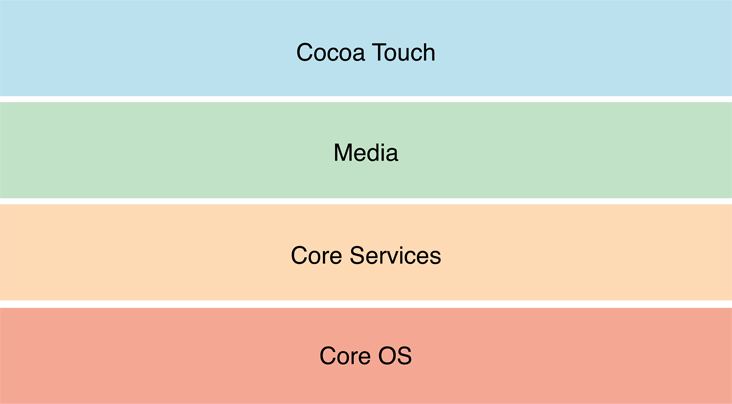
\includegraphics[width=0.7\textwidth]{pfc/figuras/ios-architecture.png}
    \caption{Camadas de abstração do sistema iOS}
    \label{fig:ios-architecture}
\end{figure}

\subsection{Ambiente de Desenvolvimento Xcode}
O Xcode é o ambiente de desenvolvimento integrado (IDE) da Apple. A ferramenta possui um editor de texto integrado, uma ferramenta de construção de interfaces (\textit{interface builder}) e outras funcionalidades que dão suporte ao desenvolvimento de aplicativos para os sistemas iOS, macOS, watchOS e tvOS. O Xcode possui o SDK iOS integrado, o qual permite a compilação, a simulação de dispositivos, entre outros recursos.

A Figura \ref{fig:xcode} ilustra a interface gráfica da IDE.
\begin{figure}[h]
    \centering
    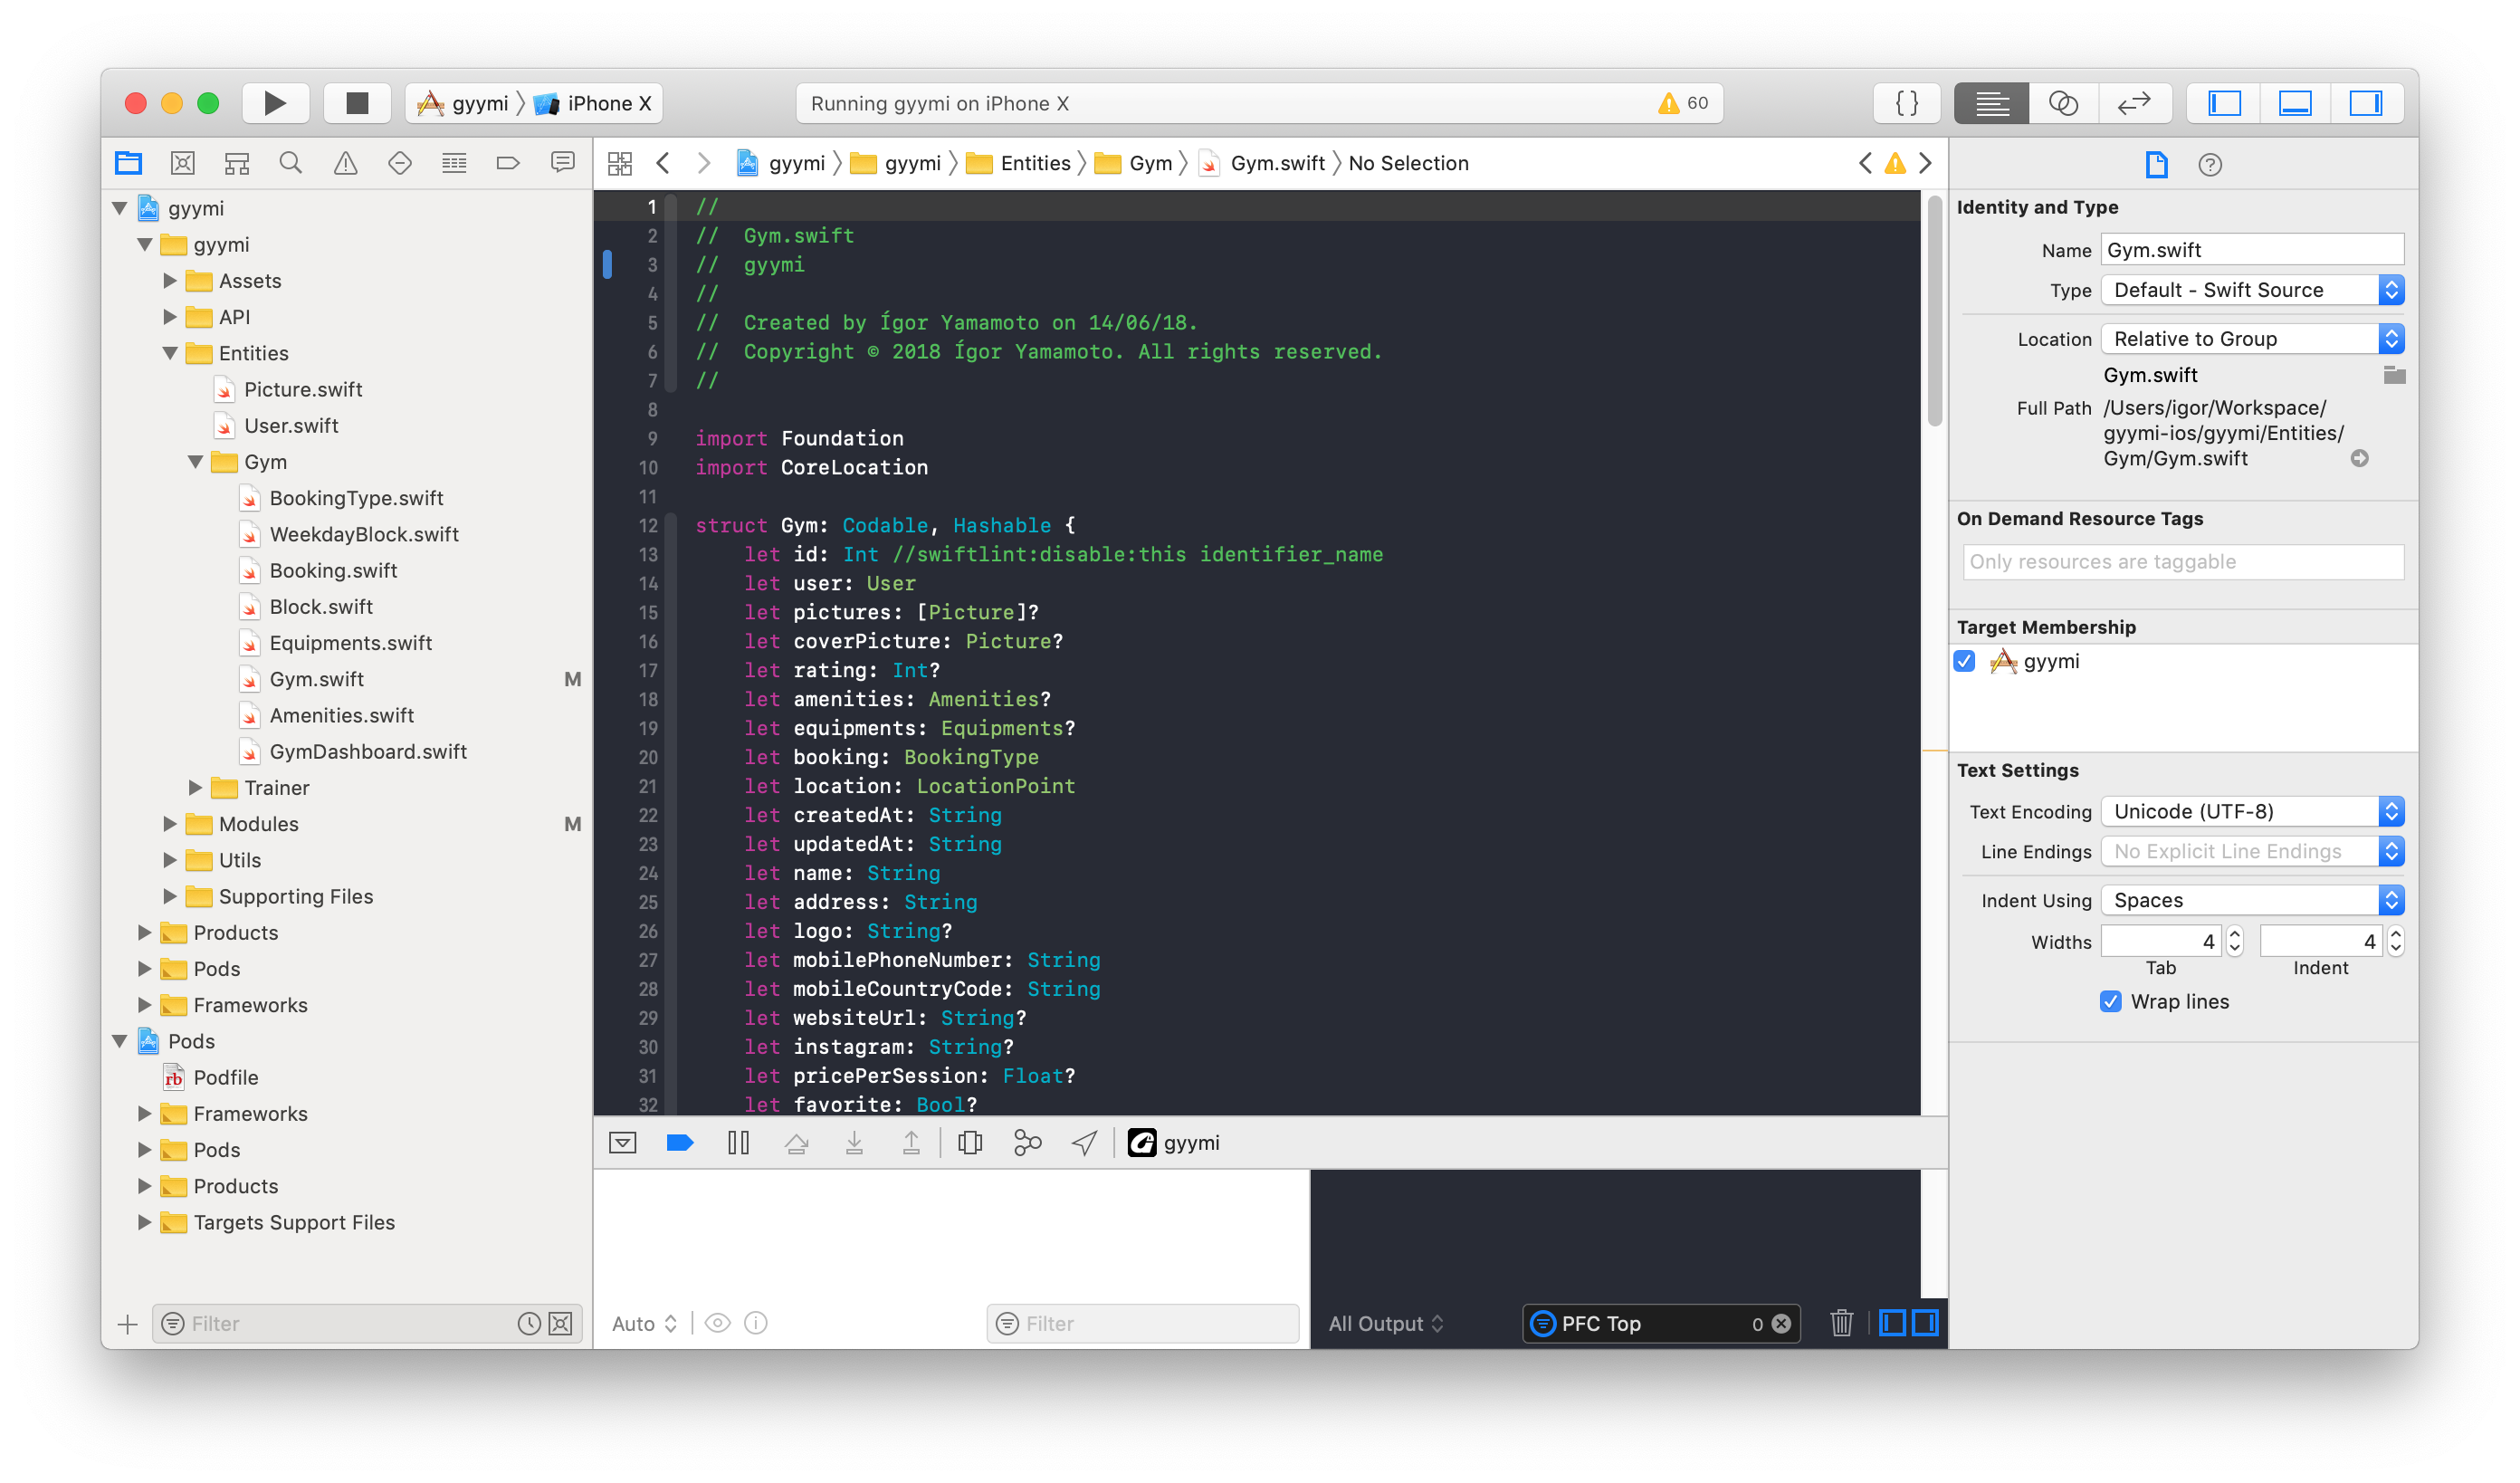
\includegraphics[width=\textwidth]{pfc/figuras/xcode.png}
    \caption{Interface gráfica da IDE Xcode}
    \label{fig:xcode}
\end{figure}

\subsection{Linguagens de Programação}
\begin{figure}[h]
    \centering
    
\includegraphics[width=0.6\textwidth]{pfc/figuras/swift.png}
    \caption{Logo da linguagem de programação Swift}
    \label{fig:swift}
\end{figure}
As linguagens de programação com suporte oficial da Apple para desenvolvimento de aplicativos nativos para iOS são Swift e Objective-C. Até a versão iOS 7 (hoje se encontra na versão 12), o Objective-C era a linguagem oficialmente utilizada. Desde o lançamento do Swift em 2014 pela Apple, a linguagem tem crescido rapidamente em popularidade e uso, aparecendo no ranking das dez primeiras linguagens de programação utilizadas por desenvolvedores \todo{citar redmonk}. A nova linguagem tem suporte para o desenvolvimento nas plataformas iOS, macOS, watchOS, e tvOS e pode ser utilizada em conjunto com o Objective-C no mesmo projeto. A compatibilidade com a antiga linguagem, permite que novos projetos em Swift utilizem bibliotecas já implementadas em Objective-C, fato que consolidou a nova linguagem como recomendada para novas aplicações.

O Swift traz diversos benefícios em relação ao Objective-C, a qual é considerada uma linguagem difícil de alcançar proficiência, tanto para programadores vindos de outras linguagens quanto para iniciantes. O Swift foi arquitetado para operar de forma segura, prevendo erros humanos, e para dar suporte as melhores práticas de programação. Algumas funcionalidades que dão suporte a essas premissas são a introdução de estruturas de dados mais sofisticadas (como tuplas) e o fato da linguagem assegurar a tipagem de dados, prevendo erros de passagem errônea de dados, e oferecer valores opcionais (\textit{Optionals}), prevendo erros de ponteiros nulos recorrentes no Objective-C por exemplo. Tendo em vista o que foi citado, a linguagem Swift foi a escolhida para o desenvolvimento do aplicativo deste trabalho.

\subsection{Gerenciamento de Dependências}
\begin{figure}[h]
    \centering
    
\includegraphics[width=0.6\textwidth]{pfc/figuras/cocoapods.png}
    \caption{Logo do gerenciador de dependências CocoaPods}
    \label{fig:cocoapods}
\end{figure}
O uso de gerenciadores de dependências, para controlar a utilização de bibliotecas externas no projeto, é um padrão para o desenvolvimento iOS. Uma das ferramentas mais frequêntes em projetos é o CocoaPods (Figura \ref{fig:cocoapods}), com mais de $53$ mil bibliotecas disponíveis e mais de $3$ milhões de aplicativos utilizando a ferramenta \todo{citar cocoapods}.

% ***********************
% Versionamento de Código
% ***********************
\section{Controle de Versão}
Controle de versão trata-se de um sistema que mantém registro de mudanças em arquivos ao longo do tempo, de forma a permitir retorno a pontos anteriores da versão dos mesmos. Um sistema de controle de versão pode ser implementado das seguinte formas \todo{citar versionamento}:

\begin{itemize}
    \item Controle Local: arquivos são copiados para outros diretórios (Figura \ref{fig:version-control-local}), sendo mantida uma versão localmente.
    \item Controle Centralizado: arquivos são mantidos em um servidor central (Figura \ref{fig:version-control-centralized}) e máquinas remotas tem a acesso as mesma versões.
    \item Controle Distribuído: arquivos são mantidos em repositórios centrais e locais (Figura \ref{fig:version-control-distributed}), de maneira a todas as máquinas possuírem uma versão completa do repositório e de seu histórico de mudanças.
\end{itemize}

\begin{figure}[h]
	\centering
    \begin{subfigure}[b]{0.3\textwidth}
      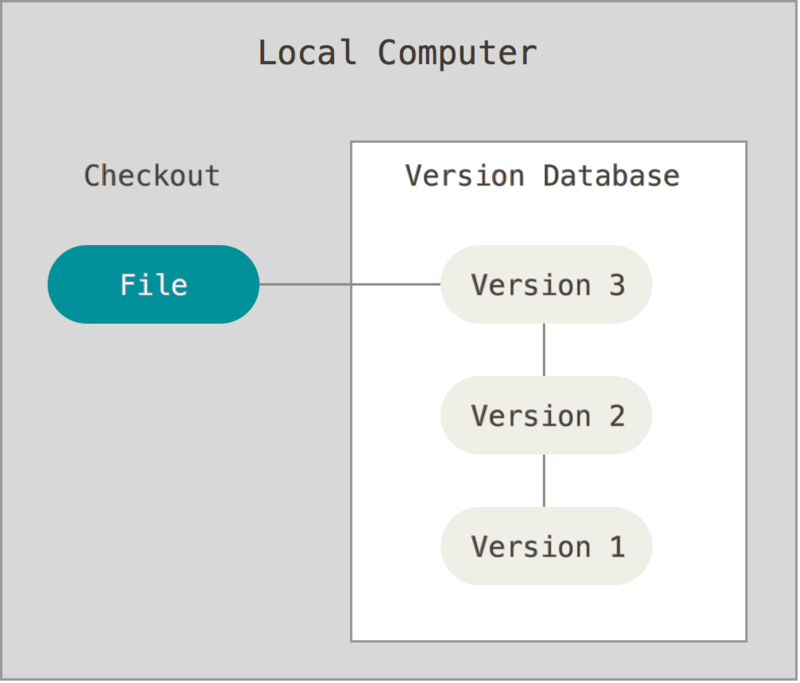
\includegraphics[width=\textwidth]{pfc/figuras/control-version-local.png}
      \caption{Controle local}
      \label{fig:version-control-local}
    \end{subfigure}
    ~
	\begin{subfigure}[b]{0.3\textwidth}
      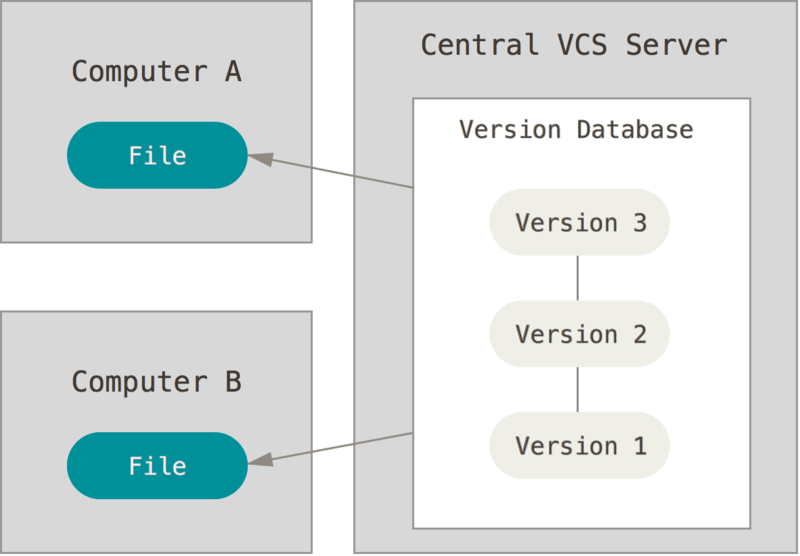
\includegraphics[width=\textwidth]{pfc/figuras/control-version-centralized.png}
      \caption{Controle centralizado}
      \label{fig:version-control-centralized}
    \end{subfigure}
    ~
	\begin{subfigure}[b]{0.3\textwidth}
       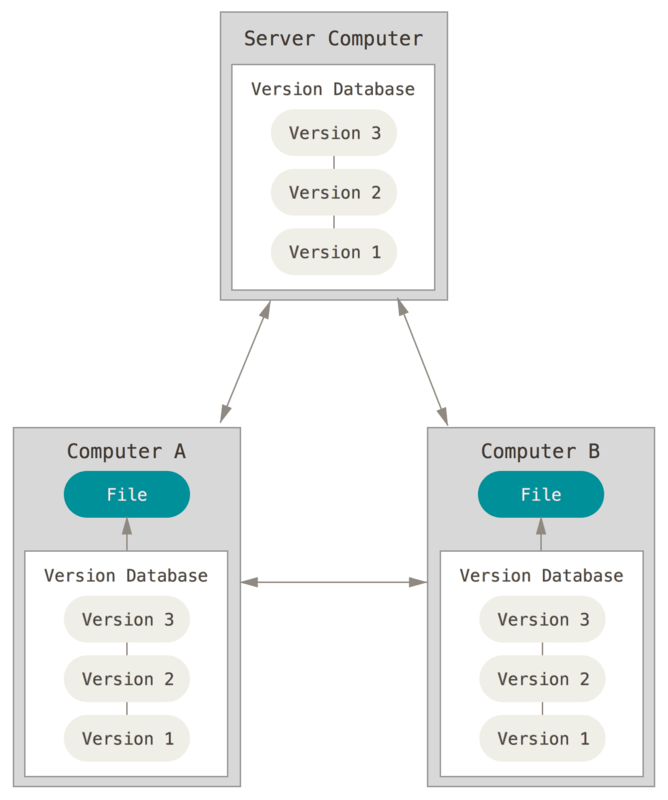
\includegraphics[width=\textwidth]{pfc/figuras/control-version-distributed.png}
       \caption{Controle distribuído}
       \label{fig:version-control-distributed}
    \end{subfigure}
    ~
    \caption{Estratégias de sistemas de controle de versão}
    \label{fig:version-control}
\end{figure}

O sistema de controle de versão distribuído traz vantagens para o trabalho conjunto de desenvolvedores, permitindo a colaboração com diferentes pessoas de forma simultânea dentro do mesmo projeto. Cada um dos desenvolvedores pode trabalhar em uma funcionalidade diferente da aplicação ao mesmo tempo em sua máquina local, a qual possui um backup completo dos dados do projeto. O sistema distribuído permite a configuração de diferentes fluxos de trabalhos que não podem ser aplicados nos sistemas locais e centralizados. Também evita problemas decorrentes dos outros sistemas, como o único ponto de falha no sistema centralizado e a dificuldade de sincronização da equipe em sistemas locais.

O sistema de controle distribuído foi utilizado no projeto através da ferramenta Git \todo{ciar git}. O Git tem sido extensivamente usado em projetos de desenvolvimento de software por todos os tamanhos de times e empresas, devido a sua facilidade de uso, performance e por se tratar de uma ferramenta de código aberto. Para gerenciamento do repositório remoto comum ao time de desenvolvimento, foi utilizado o portal GitHub \todo{citar github}. O GitHub é uma empresa que fornece serviços para facilitar o uso da ferramenta Git.

% ***********
% RESTful API
% ***********
\section{RESTful API's}
Um dos tipos mais populares de API é a baseada na arquitetura REST (\textit{Representational State Transfer}), a qual consiste em uma abstração dos elementos arquitetônicos dentro de um sistema hipermídia distribuído \todo{citar rest}. 
RESTful APIs foram projetadas para se beneficiar de protocolos existentes, utilizando o HTTP para web API's. Uma das vantagens da abordagem é o ganho de flexibilidade, já que dados não são atrelados a recursos ou métodos, permitindo a manipulação de múltiplos tipos de chamadas com diferentes formatos de retorno de dados. Esta flexibilidade permite a construção de API's que atendem a necessidade de todas as partes envolvidas no projeto. As seguintes características são observadas em RESTful API's:

\begin{itemize}
    \item Cliente e servidor devem estar separados e podem evoluir individualmente.
    \item Não armazenam estado, significando que todas as chamadas da API operam independentemente. Cada uma delas contém todos os dados necessários para serem completadas.
    \item Devido ao fator de não armazenar estado, RESTful API's são projetadas para utilizar sistemas de armazenamento em cache
    \item Possuem diferentes camadas operando em conjunto para a construção de uma hierarquia que auxilia a criação de aplicações mais escaláveis e modulaes.
    \item Não está restrita a um tipo de formato de transmissão de dados (pode transferir dados em diferentes formatos como XML e JSON). E usuários não necessitam conhecer nomes de procedimentos ou parâmetros em uma ordem específica.
\end{itemize}

% ********************
% Back-end
% ********************
\section{Back-end}

% ********************
% Testes Automatizados
% ********************
\section{Testes Automatizados}
\missingfigure{Figuras classicas dos testes, modelo em V, piramide etc}
\subsection{Testes de UI}
